\documentclass[addpoints,12pt]{exam}

\usepackage{amsmath}
\usepackage{amsthm}
\usepackage{graphicx}
\usepackage{enumitem}

\newtheorem{theorem}{Theorem}

\printanswers %Remove to hide answers
\pagestyle{headandfoot} %Adds Headers and Footers
\runningheadrule
\firstpageheader{Math 151}{Exam 1}{\today}
\runningheader{Math 151}
{Exam 1, Page \thepage\ of \numpages}
{\today}
\firstpagefooter{}{\thepage}{}
\runningfooter{}{\thepage}{}


\begin{document}

%The box at the top, and the name
\begin{center}
\fbox{\fbox{\parbox{5.5in}{\centering
Answer the questions in the spaces provided on the
question sheets. If you run out of room for an answer,
continue on the back of the page.}}}
\end{center}
\vspace{0.1in}
\makebox[\textwidth]{Name:\enspace\hrulefill}
\vspace{0.2in}

%Question Formatting
%\qformat{\textbf{Question \thequestion}\quad (\thepoints)\hfill}
%Point Table


%\begin{center}
%\gradetable[h][questions]
%\end{center}

%Beginning Questions
\begin{questions}
	\question Solve the following linear equation 
   \[
 2(x-1)+3 = x-3(x+1)~.
\]

 \begin{solution}
We seek to solve the linear equation 
   \[
 2(x-1)+3 = x-3(x+1)~.
\]
First, we can distribute the $2$ on the left side and the $-3$ on the left side. 
\[
2x-2 +3 = x - 3x -3 
\]
On the left, side, we can combine the two constant terms and the $x$-terms on the right side. 
\[
2x +1 = -2x -3
\]
Next, we can move the constant $1$ to the right, and $-2x$ to the left to get 
\[
4x = -4 
\]
Finally, we divide by both sides by $4$ to get 
\[
x = -1 
\]
 \end{solution}
 
\question Solve the following equation 
\[
 \frac{x}{5}- \frac{1}{2} = \frac{x}{6}~.
\]

\begin{solution}
	We seek to solve the following  linear equation involving fractions 
\[
 \frac{x}{5}- \frac{1}{2} = \frac{x}{6}~.
\]
    First, we can get rid of the right by multiplying by $6$. 
		\[
		 \frac{6x}{5} - \frac{6}{2} = x
	 \] 
	 Next, we can get rid of the fraction on the left by multiplying everything by $5$ 
	 \begin{align*}
		 6x - \frac{30}{2} & = 5x \\
		 6x - 15 & = 5x \\
		 6x & = 5x + 15 \\
		 x & = 15 \\
	 \end{align*}
\end{solution}

\question The length of an American football field is 200 feet more than its width. If the perimeter is 1040 feet, then how wide is the field? 
\begin{solution}
    A football field is the shape of a rectangle. Let $l$ be the length of the football field and $w$ be the width of the football field. Then, using that the length is $200$ feet longer than the width, we have 
		\[
			l = 200+w
		\]
Next, we should look at the perimeter. Note that for a rectangle, you have two sides that are the length and two that are the width. Therefore, the perimeter is 
\[
2l+2w= 1040
\]
Therefore, this problem is reduced to solving the set of linear equation 
\begin{align*}
	200 &  = l-w \\
	1040 & = 2l + 2w \\
\end{align*}
We will solve by the addtion method. Multiplying the top equation by 2 means we can solve 
\begin{align*}
	400 &  = 2l-2w \\
	1040 & = 2l + 2w \\
\end{align*}
From here, we can add the two equations together to cancel the widths 
\[1440 = 4l \]
Finally, to solve for $l$, we can dividy both sides by $4$ to get 
\[
360 = l
\]
We can then solve for $w$ by substituting $360 = l $ into the equation $l = 200 +w$
\begin{align*}
	360 & = 200 +w \\
	160 & = w \\
\end{align*}
Therefore the length of the football field is $360$ feet and the width of the field is $200 $ feet.

\end{solution}


\question You have 150 dollars to invest. Part of the money is invested in an account through Yankton Financial paying $15\%$ annual interest. The rest of the money is to be invested in a second account at Vermillian Bank paying $13\%$ interest. If you would like $\$20$ a year in interest, how much should you invest into each account? Feel free to keep your answer unsimplified. 

\begin{solution}
    Let $y$ be the amount invested in Yankton Financial and $v$ be the amount in vermillian bank. Then since the total amount we have to invest is $\$150$ 
		\[
		y+v = 150~. 
		\]
		To calculate the interest, we can convert the percentage to a decimal but dividing by $100$. Therefore, the total interest earned for both accounts is 
		\[
		0.15 y + 0.13 v = 20 
		\]
		Therefore, we must solve the system of linear equations 
		\begin{align*}
			y+v & = 150 \\
			0.15 y + 0.13 v & = 20 \\
		\end{align*}
		In order to solve, we can multiply the first equation by $-0.15$ to get 
			\begin{align*}
			-0.15y+-0.15v & = -22.5 \\
			0.15 y + 0.13 v & = 20 \\
		\end{align*}
		Adding the two equations together gives 
		\[
			-0.02 v  = -2.5
		\]
		Therefore, if we multiply both sides by $-50$ we get 
		\[
		v = 125
		\]
		Therefore, since $y+v = 150$, we can solve for $y$ 
		\[
		y = 150 - 125 = 25
		\]
		Therefore, we should invest $\$25$ into yankton financial and $\$ 125$ into Vermillion Bank. 
\end{solution}

\question Perform the following computation using complex numbers. 
   \[
		 (7+2i)-(5-7i)= 
\]

\begin{solution}
	Recall, that to add or subtract complex numbers, we can add or subtract the real parts and the imaginary parts seperately
    \begin{align*}
			(7+2i) - (5-7i) & = (7-5) + (2i - (-7i)) \\
			 & = (7-5) + (2i +7i)\\
			 & = 2 + 9i \\
    \end{align*}
\end{solution}



\question Perform the following computation using complex numbers. 
\[
		 (3+5i)(-5-i)=
\]
\begin{solution}
    Recall, that to multiply complex numbers we can distribute (FOIL) them like polynomials. Remember as well that $i^2 = -1$ as well, which we can use to simplify after we distribute. 
\begin{align*}
    (3+5i)(-5-i) & = -15 -3i -25i -5i^{2}\\
		 & =  -15 - 3i - 25i +5 \\
		 & = (-15+5) + (-3i-25i) \\
		 & = -10 -28 i \\
\end{align*}
\end{solution}

\question Solve the following quadratic equation by factoring~. 
\[
	x^{2}-3x-10=0 
\]

\begin{solution}
    We can begin factoring by looking for two numbers $a$ and $b$ such that $a*b = -10$ and $a+b = -3$. Noting that $-5*2=10$ and $-5+2 = -3$, we can factor the polynomial as follows.  
		\[
			(x-5)(x+2) = x^{2}-3x-10 = 0 
		\]
		Therefore, the solutions are given by the pair of equations 
		\[
		x-5 = 0 \hspace{30pt} x+2 = 0 
		\]
		Therefore, $x=5$ and $x=-2$ are the two solutions to the quadratic equation. 
\end{solution}

\question Solve the following quadratic equation by the square root property. 
   \[
   5x^{2}+1=26
   \]

	 \begin{solution}
	     Since there is no degree $1$ term, we can solve directly (square root property). 
			 \begin{align*}
				 5x^{2}+1 & = 26 \\
				 5x^{2} & = 25 \\
				 x^{2} & = 5 \\
				 x & = \pm \sqrt{5}\\
			 \end{align*}
			 Therefore the two solutions are $x = \sqrt{5}$ and $x = -\sqrt{5}$
	 \end{solution}
\question Solve the following quadratic equation by using the quadratic formula (Formula on Last Page)
   \[
x^{2}+6x-7=0
\]

\begin{solution}
    The quadratic equation states that the solutions are given by 
		\[
		x = \frac{-b\pm \sqrt{b^{2}-4ac}}{2a}
		\]
		where $a = 1$, $b = 6$, and $c = -7$. Therefore the two solutions are given by 
		\[
		x = \frac{-6\pm \sqrt{6^{2}-4*1*(-7)}}{2}
		\]
\end{solution}
\question Solve the following equation involving radicals~.
   \[
    \sqrt{2x-1}=x
	 \]
\begin{solution}
    We can begin by squaring both sides of the equation to get 
		\[
		2x-1 = x^{2}
		\]
		We can then isolate the quadratic equation on one side, and then factor 
	\begin{align*}
	    0 = & x^{2}-2x+1 \\
			0 & = (x-1)^{2} \\
	\end{align*}
	Therefore $x=1$ is the solution to the quadratic equation.
\end{solution}
	     

	 \question Solve the following equation involving rational exponents 
	    \[
	  7|x-3|+2=16
	 \]

\begin{solution}
    First, we can isolate the absolute value on the left side
		\begin{align*}
		    7|x-3| = 14 \\
				|x-3| = 2 \\
		\end{align*}
		Next, we can splity into two equations 
		\[
		x-3 = 2 \hspace{30pt} x-3 = -2 
		\]
		Therefore, the two solutions are $x =5 $ and $x = 1 $ . 
\end{solution}

\question Give each interval in interval notation 
\begin{enumerate}[label = \alph*)]
    \item $ 1 < x \leq 6$  
		\item $ x\geq 2  $
		\item $-2 \leq x \leq 5 $ 
		\item $x \leq -2 $ 
\end{enumerate}


\begin{solution}
\begin{enumerate}[label = \alph*)]
	\item $(1,6]$
	\item $[2,\infty)$
	\item $[-2,5]$
	\item $(-\infty,-2)$
\end{enumerate}
\end{solution}

\question Solve the linear inequality
   \[
4(x+1)+2\geq 3x-13
\]

\begin{solution}
    First, we can distribute the $4$ to get 
		\[
		4x + 4 +2  \geq 3x - 13 \\
		\]
		We have two constants on the left side, so we can simplify. 
		\[
		4x + 6 \geq 3x - 13 \\
		\]
		Next, in order to keep the $x$ terms positive, we can move the $3x$ to the left, and the $6$ to the right side. 
		\[
		x \geq -19  \\
		\]
	  Therefore, $x$ must be in the interval $[-19,\infty)$ 
\end{solution}

\question Solve the absolute value inequality 
\[
|3x-9| > 3
\]

\begin{solution}
    We can solve the two equations 
		\[
		3x - 9 > 3 \hspace{30pt} 3x - 9 < -3 
		\]
		First, solving the left equation, we get 
		\begin{align*}
		    3x - 9 & > 3 \\
				4x & > 12 \\
				x & > 3 \\
		\end{align*}
		Solving the right equation gives 
		\begin{align*}
			3x - 9 & < -3 \\
			3x  & < 6 \\
			x & < 2 \\
		\end{align*}
		Therefore, it must be the case that either $x <2 $ or $x >3$ . Therefore $x$ must be in the interval 
		\[
			(-\infty,2) \cup (3, \infty)
		\]
\end{solution}

\question Solve the system of linear equations

\begin{align*}
	x&+3y=8\\
	2x&-y=9\\
\end{align*}

\begin{solution}
    By isolating $y$ in the second equation, we get 
		\[
		2x - 9 = y 
		\]
		We can substitute $y$ into the first equation to get 
		\[
		x + 3(2x - 9 ) = 8 
		\] 
		From here, we can solve to find $x$ 
		\begin{align*}
			x + 3(2x-9) & = 8 \\
			x + 6x -27 & = 8 \\
			7x & = 35 \\
			x & = 5 \\
		\end{align*}
		Substituting this into the second equation to solve for $x$ gives 
		\begin{align*}
		    2x - 9 & = y \\
				2*5 -9 & = y \\
				10 - 9 & = y \\
				1 & = y \\
		\end{align*}
		Therefore, the intersection point of the two lines is $(5,1)$. 
\end{solution}

\question Solve the system of linear equations 
\begin{align*}
	x&+2y=2 \\
		-4x&+3y = 25 \\
\end{align*}

\begin{solution}
    Multiplying the first equation by $4$ gives 
\begin{align*}
	4x&+8y=8 \\
		-4x&+3y = 25 \\
\end{align*}

From here, we can add the two equations together to elimiate the $x$'s 
\[
11 y = 33 
\]
Which gives that $y=3$. Substituing this into the first equation gives 
\begin{align*}
	x + 2(3) & = 2 \\
	x & = -4 \\
\end{align*}

Therefore, the intersection point is $(-4,3)$. 

\end{solution}


\question Use the graph to evaluate the following function

\[
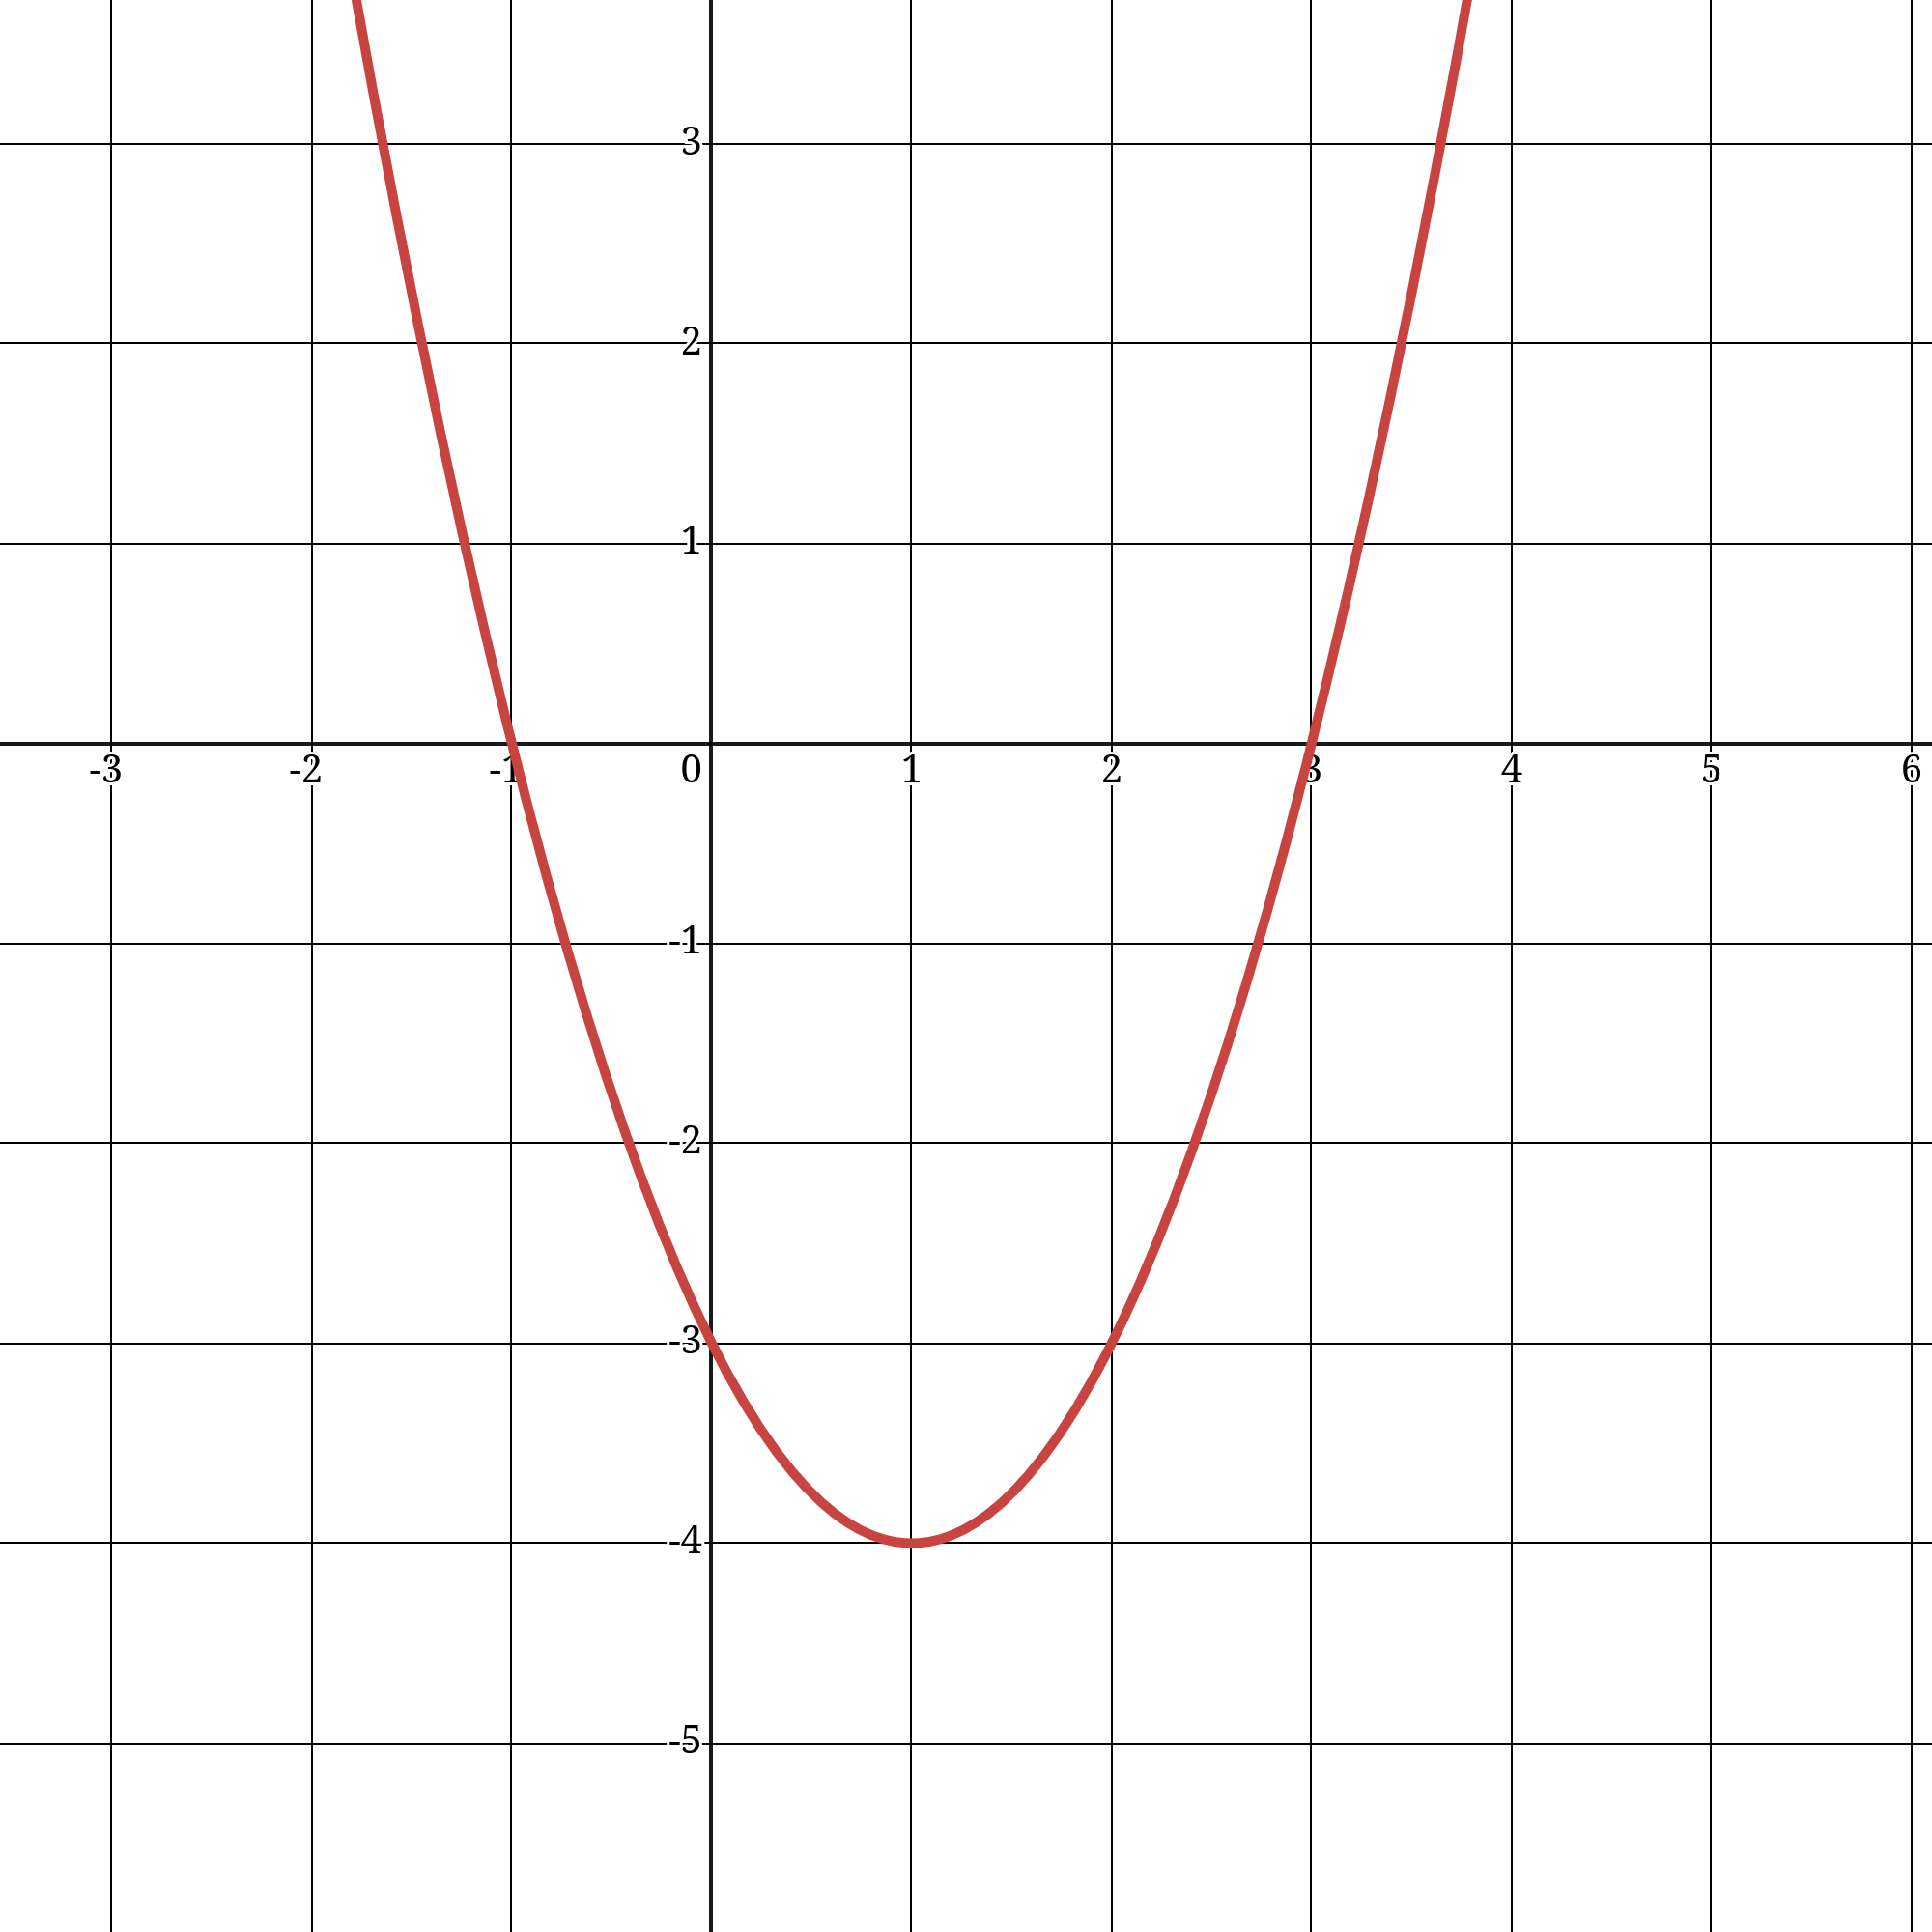
\includegraphics[scale = 0.1]{quadratic_graph}
\]

\begin{enumerate}[label = \alph*)]
    \item $f(-1) =   $
		\item $f(0) =  $
		\item $f(1) = $
		\item $f(2) = $
\end{enumerate}

\begin{solution}
\begin{enumerate}[label = \alph*)j]
    \item $f(-2) = 0$
		\item $f(0) = -3$
		\item $f(1) = -4$
		\item $f(2) = -3$
\end{enumerate}
\end{solution}

\question Evaluate the function
\[
f(x)=x^{2}+2x+3
\]
for the following function values 
\begin{enumerate}[label = \alph*)]
    \item $f(-2)=$ 
		\item $f(x+1)=$
		\item $f(-x)=$
\end{enumerate}

\begin{solution}
     \begin{enumerate} [label = \alph*)]
         \item $f(-2) = (-2)^{2} + 2(-2) +3 $
				 \item $f(x+1) = (x+1)^{2}+2(x+1)+3 $
				 \item $f(-x) = (-x)^{2}+2(-x)+3 $
     \end{enumerate}
\end{solution}

\question Find the relative maximum and minimums of the following graph 

\begin{figure}[htb!]
  \centering
  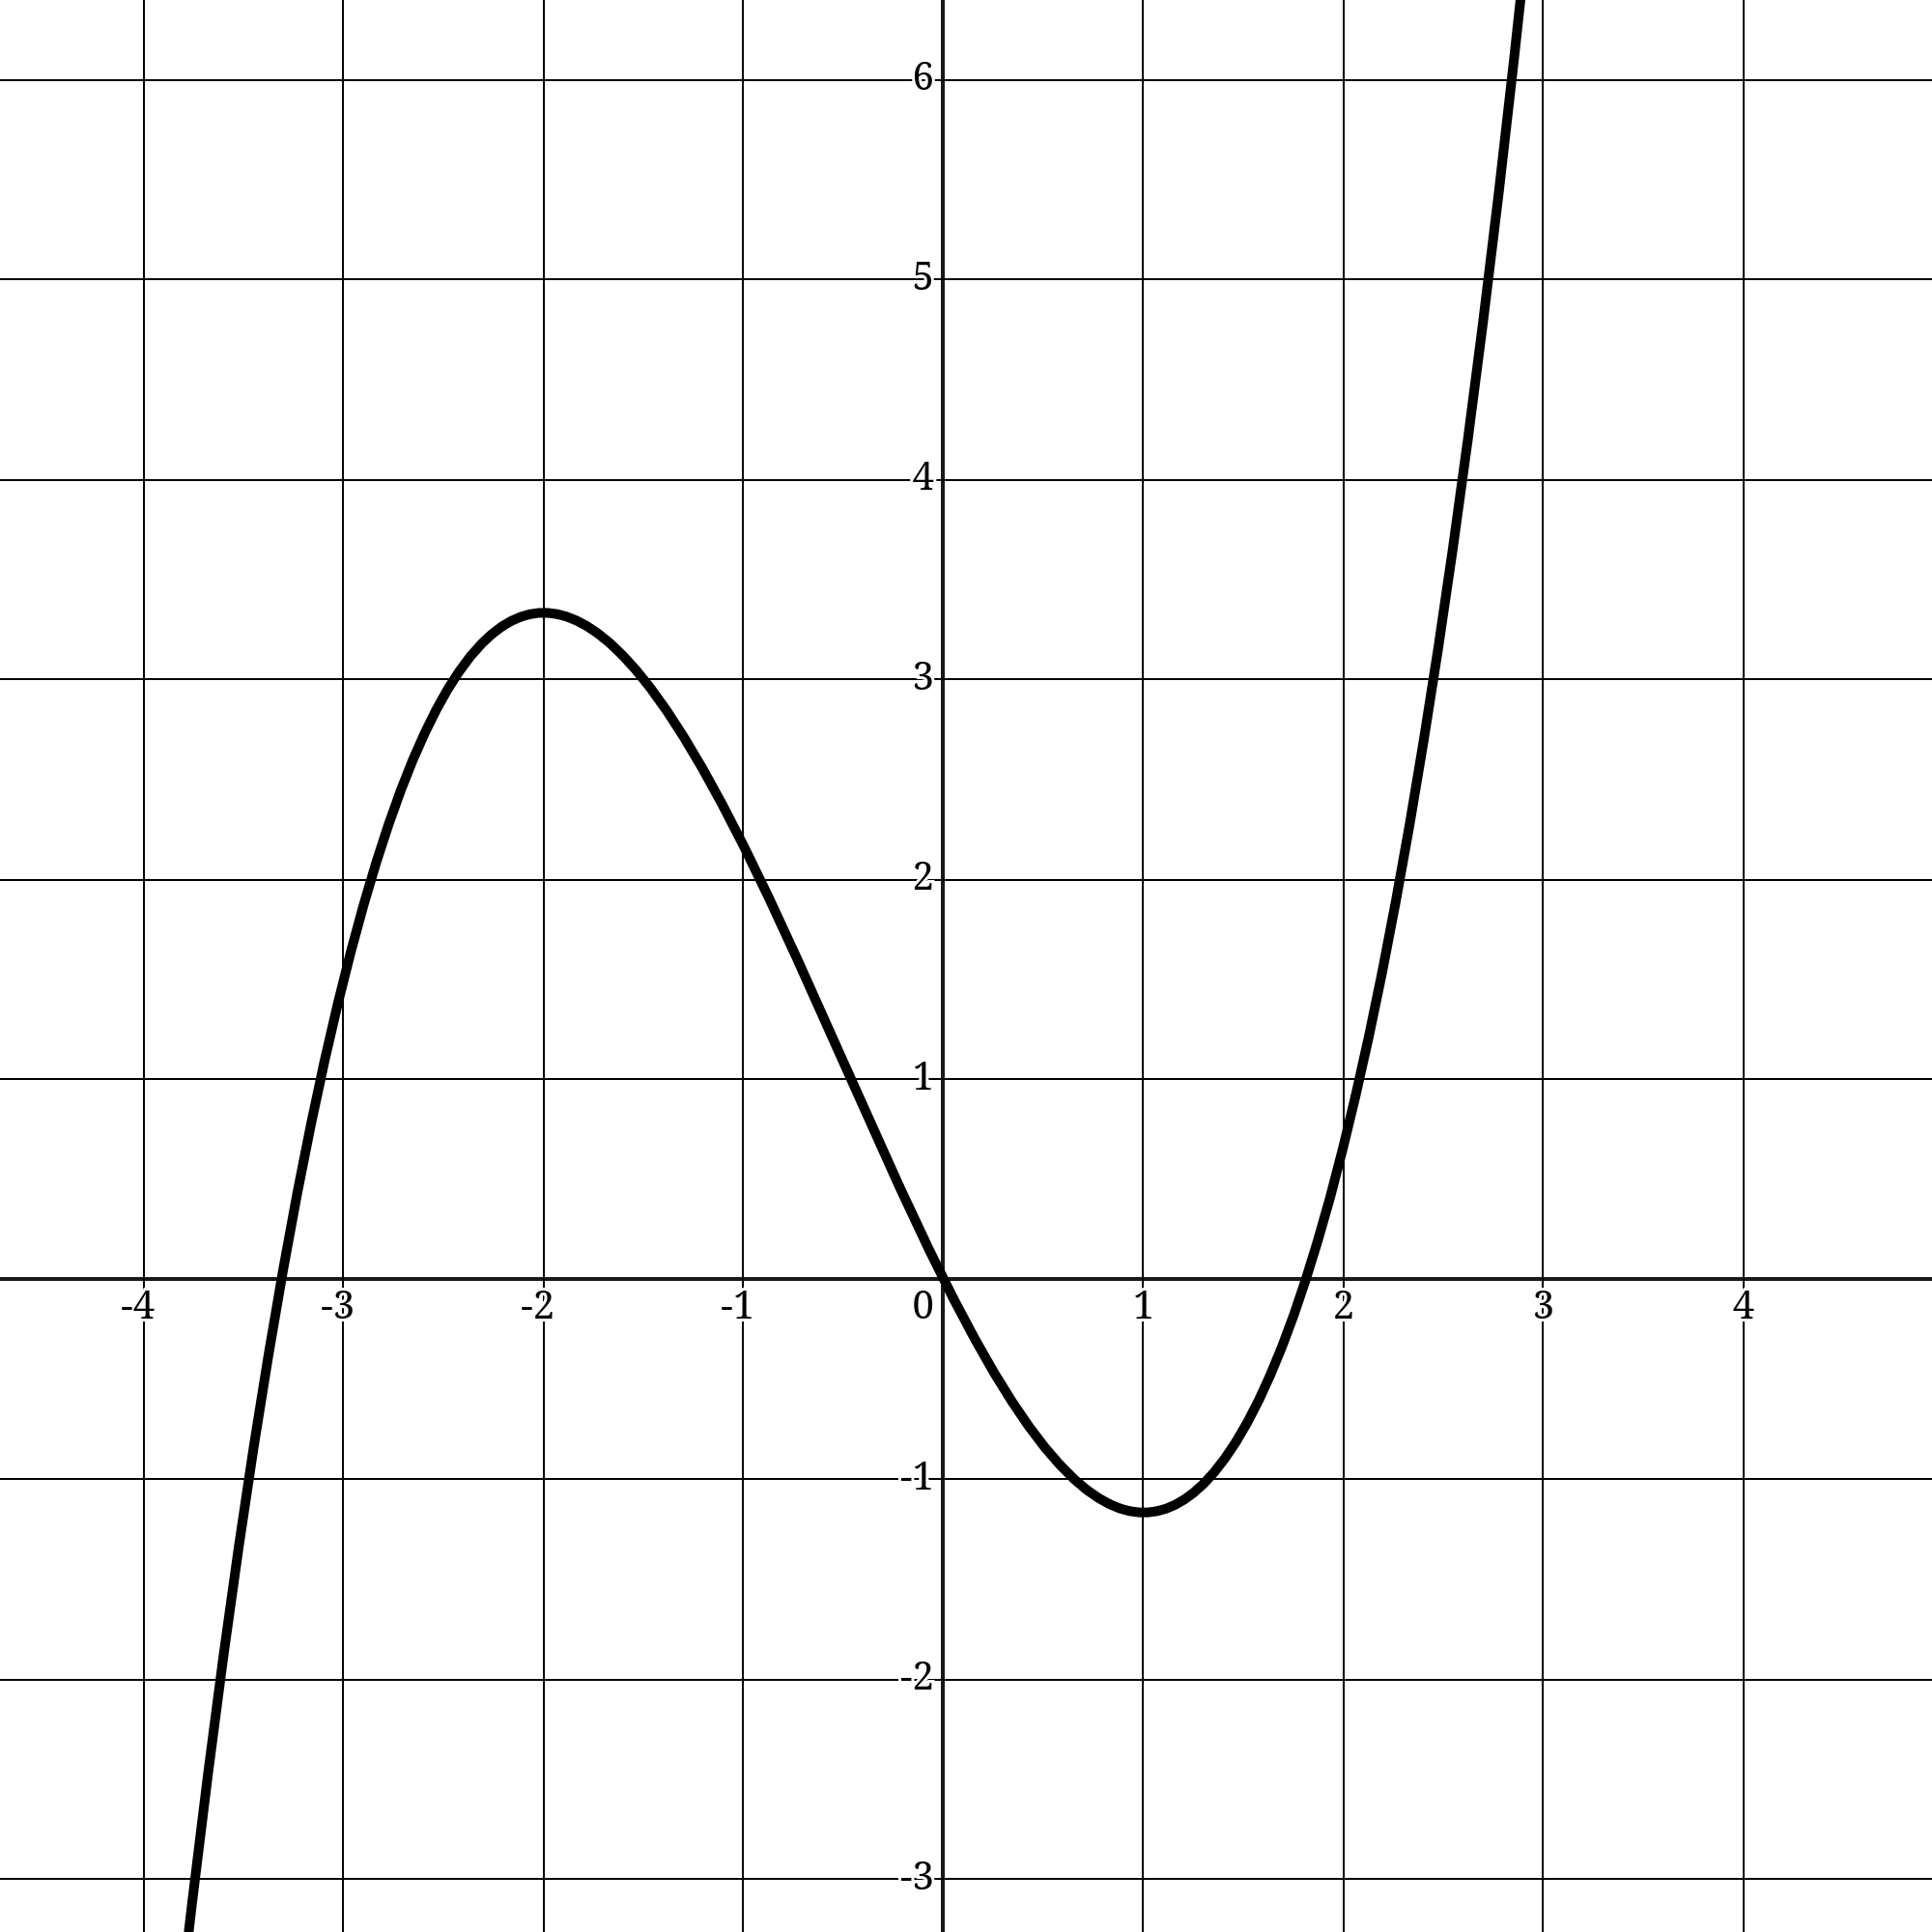
\includegraphics[scale = 0.1]{minmax}
\end{figure}

\begin{solution}
    There is a relative minimum at $x =1 $ The relative minimum value is at about $y = -1.2 $. I will not be super specific with you needing to get $-1.2$ here. Your best guess between $-1$ and $-2$ will do. There is a relative maximum at $x = -2$. The relative maximum value is about  $y = 3.3$. Again, any value between $3$ and $4$ will do. Note that this is why algebraic equations are nice, if we had the algebraic formula, we could just compute $f(1)$ and $f(-2)$. 
\end{solution}

\question Give an example of an even function, and verify that it is an even function. 

\begin{solution}
	An example of an even equation is $f(x)= x^{2}$. This is even since $f(x) = f(-x)$, as $f(-x) = (-x)^{2} = x^{2}$
\end{solution}

\question Evaluate the following piecewise function at the following values
\[
	f(x) =
	\begin{cases}
   x+4 & x\leq -3 \\
	 -x+2 & x> -3 \\
	\end{cases}
\]

\begin{enumerate}[label = \alph*)]
    \item $f(-5)=$
		\item $f(-3) = $
		\item $f(-1)= $
		\item $f(0)=$
\end{enumerate}

\begin{solution}
    \begin{enumerate}
        \item $-5 \leq -3$, so we can use the first equation to get \[
        f(-5) = -5 +4 = -1 
        \]
			\item $-3 \leq -3$ (after all $-3 = -3$), so we can use the first equation to compute \[f(-3)= -3+4 =1 \]
			\item $-1 > -3 $ , so we can use the second equation to compute 
				\[
				f(-1) = -(-1)+2 = 3 \\
				\]
		\item $0>3$, so we can use the second equation to compute \[f(0) = -0+2 = 2 \]
    \end{enumerate}
\end{solution}

\end{questions}

\begin{theorem}
    Let $ax^{2}+bx +c =0$ be a quadratic equation. Then the solutions to the quadratic equation are given by 
		\[
		x = \frac{-b \pm \sqrt{b^{2} - 4ac}}{2a}
		\]
\end{theorem}

\end{document}
